La figura mostra la gràfica de la \textbf{funció derivada} $f'$ d'una funció $f$ definida a
tot $\mathbb{R}$.

\begin{center}
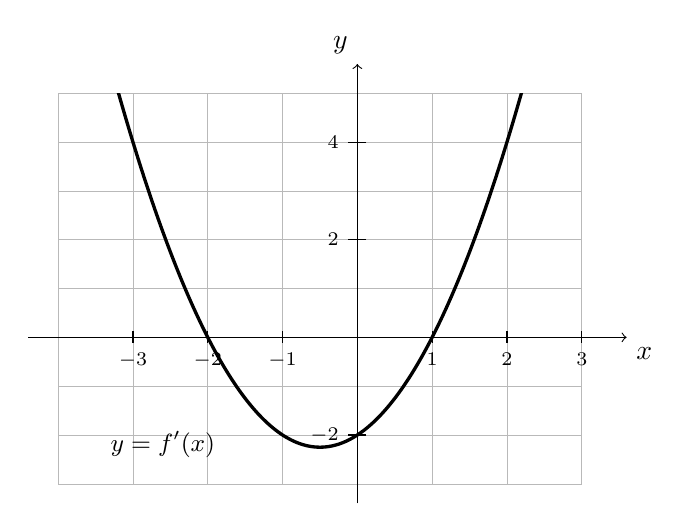
\begin{tikzpicture}[x=0.95cm,y=0.62cm]
  \draw[gray!55,very thin,step=1] (-4,-3) grid (3,5);
  \draw[->] (-4.4,0) -- (3.6,0) node[below right] {$x$};
  \draw[->] (0,-3.4) -- (0,5.6) node[above left] {$y$};
  \foreach \i in {-3,-2,-1,1,2,3} \draw (\i,0.12) -- (\i,-0.12) node[below,font=\scriptsize] {$\i$};
  \foreach \j in {-2,2,4} \draw (0.12,\j) -- (-0.12,\j) node[left,font=\scriptsize] {$\j$};
  \begin{scope}
    \clip (-4,-3) rectangle (3,5);
    \draw[\colorgrafica,very thick,domain=-3.6:2.6,samples=90,smooth] plot (\x,{(\x+2)*(\x-1)});
  \end{scope}
  \node[\colorgrafica,font=\small] at (-2.6,-2.2) {$y=f'(x)$};
\end{tikzpicture}
\end{center}

\begin{apartats}

\apartat[1,25]{1}
A partir de la gràfica, digues on creix i on decreix $f$, i on té extrems relatius i de quin
tipus.

\begin{solucio}
$f'$ s'anul·la en $x=-2$ i en $x=1$, és positiva fora de $[-2,1]$ i negativa a dins.\\
Per tant, $f$ \textbf{creix} a $(-\infty,-2)$, \textbf{decreix} a $(-2,1)$ i \textbf{creix} a
$(1,+\infty)$.\\
En $x=-2$, $f'$ passa de positiva a negativa: \textbf{màxim relatiu}.\\
En $x=1$, de negativa a positiva: \textbf{mínim relatiu}.
\end{solucio}

\begin{nomesllarg}
\apartat{0,75}
Comprova que la funció
\[
f(x)=\frac{x^3}{3}+\frac{x^2}{2}-2x+1
\]
té aquesta derivada, i calcula el valor dels seus extrems relatius.

\begin{solucio}
$f'(x)=x^2+x-2=(x+2)(x-1)$: és la paràbola de la figura.\\
$f(-2)=-\dfrac83+2+4+1=\dfrac{13}{3}$ i $f(1)=\dfrac13+\dfrac12-2+1=-\dfrac16$.\\
Màxim relatiu $\left(-2,\tfrac{13}{3}\right)$ i mínim relatiu $\left(1,-\tfrac16\right)$.
\end{solucio}
\end{nomesllarg}

\apartat[1,25]{0,75}
Quants punts amb recta tangent horitzontal pot tenir, com a màxim, una funció polinòmica de
grau $3$? Raona-ho.

\begin{solucio}
La tangent és horitzontal on $f'(x)=0$. Si $f$ té grau $3$, aleshores $f'$ té grau $2$ i, com
a màxim, dues arrels reals: per tant, \textbf{com a màxim dos punts}.\\
Poden ser dos (com a la figura), un de sol (arrel doble) o cap.
\end{solucio}

\end{apartats}
